%
% 総合研究概要書原稿サンプルファイル
%
% ・題名,  研究室名, 学籍番号, 氏名, 指導教員名 は1段組,
%   本文は2段組.全体で1ページ。ページ番号は不要。
% ・カラー使用可だが,PDF化したときにファイルサイズが最大 5MB 程度に収まるようにすること。
% ・余白, フォントサイズなどは多少変えてもよいが, あまり大幅に
%   変更しないように.他の人の概要とのバランスも考えて.
%
\documentclass[twocolumn]{jarticle}
\usepackage{amsmath,amsfonts,amssymb}
\usepackage{color}
\usepackage[dvipdfm]{graphicx}
\usepackage{booktabs}

\pagestyle{empty}
\setlength\textheight{255mm}
\setlength\textwidth{170mm}
\setlength\topmargin{-5mm}
\setlength\oddsidemargin{-5mm}
\setlength\headheight{0mm}
\setlength\headsep{0mm}
\setlength\columnsep{8mm}
%**************************
\title{
  \LARGE\bf
  総合研究概要書原稿サンプ \\[1ex]}
\author{応用数理研究室 \quad
        BV????? 数理 科太郎 \quad
        指導教員 大宮 シス子 教授}
\date{}
%**************************
\begin{document}
\maketitle
\thispagestyle{empty}

\section{はじめに}
これはシステム理工学部数理科学科の総合研究概要書のサンプルです.
このフォーマットを参考にして作成してください.
おおむねこのような形式に従っていれば多少の変更は問題ありません.
詳細は指導教員の指示に従ってください.


\section{箇条書きの例}
\subsection{番号付き}
\begin{enumerate}
\item 数値・数式処理システムの開発・解析・応用
\item 非線形偏微分方程式の逆問題解析
\item 数理形態学による画像処理
\end{enumerate}
\subsection{番号なし}
\begin{itemize}
\item コンピュータをもっともっと進化させたい
\item ソフトウェアをもっと使いやすくしたい
\end{itemize}



\section{図の挿入}
図の挿入には \verb!\includegraphics! を使うのが一般的です.
\begin{figure}[h]
 \begin{center}
  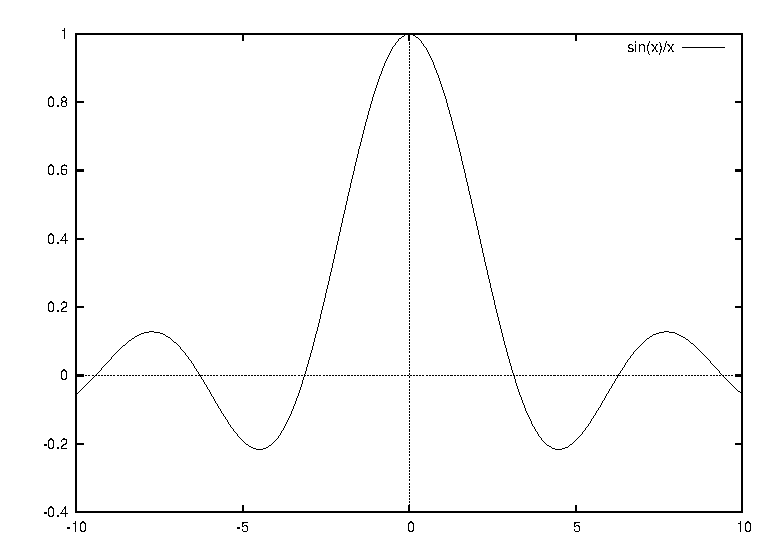
\includegraphics[width=55mm,height=45mm,keepaspectratio]{fig.eps}
  \caption{図のキャプションは図の下側に配置.}
  \label{fig:test}
 \end{center}
\end{figure}
\verb!figure! 環境を使うと, 図をフロートして (浮かせて),
適当な位置に配置してくれます.表も同様 (\verb!table! 環境).



\verb!\label! を指定しておけば,\verb!\ref! で図番号の引用も可能.
例えば,
``図\ref{fig:test}は {\tt gnuplot} による'' など (ダブルクォーテーション
の書き方も注意).表番号も同様 --- 表\ref{tbl:test}は点数表 --- ですが,
\verb!\caption! が自動生成する図番号と表番号はデフォルトでは別系統になっています (それぞれ 1 から始まって,別個に増加する).

\section{参考文献の参照}
参考文献の参照も同様 (\verb!\bibitem! で指定したラベルを \verb!\cite! で呼び出し).
例えば,阿部先生,古城先生達が書かれた数値解析の教科書\cite{Abe92}参照,など。

  ただし, \LaTeX\ は1パスコンパイラ (タイプセッタ) であり, ラベル・図番等
の引用は外部ファイル {\tt ???.aux} を通して行っている関係で, これらを
正しく処理するにはコンパイル (タイプセット) を2回以上かける必要があります.



\section{その他}
概要集をは電子データでの提出なので,
\color{blue}カ\color{green}ラ\color{red}ー\color{cyan}を使っても
\color{magenta}構いません\color{black}.
\par
なお, このサンプルは2ページ目の半分以下で終わってしまいますが,
皆さんは2ページ右の段までほぼ埋まるくらい,バランスよく書くよう
心がけてください.参考文献も忘れずに.
その他,\LaTeX\ の使い方は各自で学んでください.
\par

\begin{thebibliography}{1}
\bibitem{Abe92}
  阿部剛久 他, 数値解析入門, 昭晃堂, 1992.
\bibitem{Shibata04}
  柴田徹太郎, Three-term spectral asymptotics for the perturbed simple
  pendulum problems, 日本数学会2004年度秋季総合分科会関数方程式論分科会
  講演アブストラクト, 22--23.
  % TeX の字の文で, - はハイフン, -- は範囲を表す線, --- は本文から
  % 少し外れた内容を書くときに括弧のようにして使う線として扱われる.
\bibitem{Shibata02}
  T.Shibata, Precise spectral asymptotics for the Dirichlet problem
  $-\triangle u=\lambda\sin u$, J.Math.\ Anal.\ Appl., {\bf 267}
  (2002), 576--598.
\bibitem{Web1} {\tt http://www.sic.shibaura-it.ac.jp}
  % URL を書くときはタイプライタ体 {\tt ...} を用いるとちょっとかっこいい.
\end{thebibliography}
\end{document}  	  

